\section{Empirical Analysis of Capability Loss}
\label{sec:observed}

\subsection{\texorpdfstring{\rev{Responses to Pruning and Quantization}}{Responses to Pruning and Quantization}}
\label{sec:resp_capabilities}\label{sec:state_config}

\rev{Compression changes capabilities unevenly and in no fixed order (Fig.~\ref{fig:heterogeneity}), which is
the first structure a predictor has to capture. On the controlled Pythia panel, mathematics and code
share one shape in density with a capability-specific scale, whereas the question-answering response
changes sign across density at every state (Appendix Fig.~\ref{fig:pythia_responses}). The two
compression axes also carry different shapes. Under pruning, once the measured first-order alignment
term is subtracted, the residual before the cliff is a power law in the deleted capability mass, with an
exponent that transfers across families. Under quantization the response is instead a threshold in bit
width whose position depends on the group size, so an interpolation over the measured grid predicts it
where a smooth surface does not. Both accounts read measurements of the compressed model, so they
explain rather than predict (Appendix~\ref{sec:app_mech}).}

\begin{figure}[t]
\centering

\includegraphics[width=\textwidth]{figs/fig8_legend.pdf}\\[1pt]
\begin{subfigure}[t]{2.7in}\centering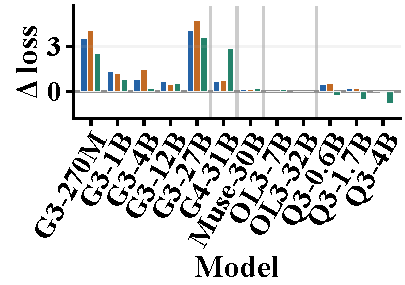
\includegraphics[width=\linewidth]{figs/fig8_a.pdf}\caption{Pruning at $d=0.7$}\end{subfigure}\hfill
\begin{subfigure}[t]{2.7in}\centering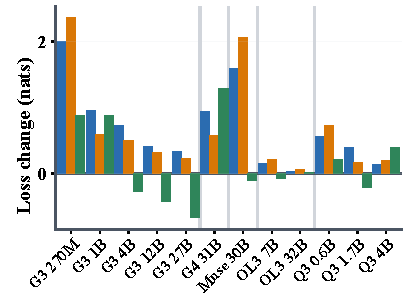
\includegraphics[width=\linewidth]{figs/fig8_b.pdf}\caption{Per-channel int4}\end{subfigure}
\caption{Capability loss change from each model's dense loss across twelve public models, under (a) pruning to $d=0.7$ and (b) per-channel int4. The ordering of capabilities changes across series and the magnitudes differ by two orders of magnitude at the same setting.}
\label{fig:heterogeneity}
\end{figure}
Model state sets the scale of the pruning response for mathematics and code, and the quantization response depends on the full configuration. On Pythia checkpoints whose size and training stage vary independently, parameter count and
pretraining tokens enter the pruning amplitude for mathematics and code and carry those capabilities to unseen densities of states that
entered the fit; the same inputs over-predict question answering, whose density response is not
proportional to any shared curve. A per-setting regression on parameter count, pretraining tokens and reference loss
reduces the mean absolute error from 0.41 to 0.25 nats for mathematics and from 0.52 to 0.29
for code, and raises it from 0.50 to 0.81 for question answering. Under quantization the configuration acts through two axes at once, the threshold in bit width
moving with the group size, so a relation needs the configuration in full and the initial state only
where it helps.

\subsection{Effects of Training Data and Evaluation Distribution}
\label{sec:why}

\rev{The cost of heavy data reuse recurs across question-answering distributions, while the net benefit of
distillation depends on the evaluation distribution. At a matched budget $T$ near 200k supervised tokens
(Fig.~\ref{fig:responses_v2}), a reuse ratio $E=T/D_U$ near twelve costs question answering $+0.29$,
$+2.55$ and $+4.85$ nats on students of 100M, 700M and 3.2B non-embedding parameters, and nine times
more independent data converts the same budget into a gain near one nat on each. Rescored on a fresh
2Wiki sample, on MuSiQue and on TriviaQA at the same budget, all three distributions worsen at high
reuse and improve as reuse falls, but only the fresh 2Wiki sample crosses into a gain. The reuse
response also fixes an empirical data requirement: a pre-specified experiment of eighteen trajectories
on the 1B and 4B students, with pools from 9k to 158k supervised tokens and three evaluation budgets,
measured the range of independent data at which a loss constraint is met (Appendix
Fig.~\ref{fig:dreq}). It is crossed inside the tested pools on the fresh 2Wiki sample for
both students at the two larger budgets, on MuSiQue only at looser tolerances, and on TriviaQA not at
all for the 4B student, where the requirement is a lower bound; because a low-degree boundary relation
did not predict these ranges better than a per-student monotone interpolation, we report measured
intervals.}

\rev{The training recipe is a further condition to consider when extending these relations. With every
other setting held fixed (Appendix Fig.~\ref{fig:lr_pilot}), the loss increase on mathematics and code
grows by an order of magnitude between learning rates of $5\times10^{-5}$ and $1\times10^{-4}$; at the
lower rate the 1B student is almost unharmed on those two capabilities and question answering improves
by $0.79$ nats, so the responses of Fig.~\ref{fig:responses_v2} are measured under one fixed recipe.
These responses motivate predictors that account jointly for data availability and training exposure,
with student state and evaluation distribution determining their range of transfer.}
